\tikzset{every picture/.style={line width=0.75pt}} %set default line width to 0.75pt        

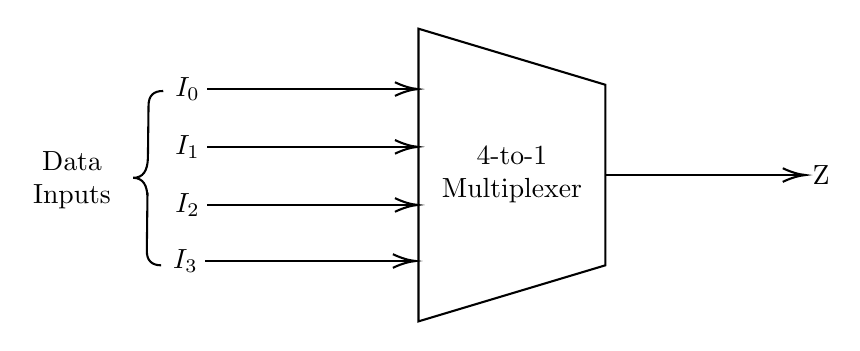
\begin{tikzpicture}[x=0.75pt,y=0.75pt,yscale=-1,xscale=1]
%uncomment if require: \path (0,642); %set diagram left start at 0, and has height of 642

%Shape: Trapezoid [id:dp36780303890607047] 
\draw   (223,53) -- (313,80) -- (313,167) -- (223,194) -- cycle ;
%Straight Lines [id:da433567050769597] 
\draw    (121.16,82.08) -- (220.58,82.08) ;
\draw [shift={(222.58,82.08)}, rotate = 180] [color={rgb, 255:red, 0; green, 0; blue, 0 }  ][line width=0.75]    (10.93,-3.29) .. controls (6.95,-1.4) and (3.31,-0.3) .. (0,0) .. controls (3.31,0.3) and (6.95,1.4) .. (10.93,3.29)   ;
%Straight Lines [id:da5507483232198851] 
\draw    (120.16,164.92) -- (219.58,164.92) ;
\draw [shift={(221.58,164.92)}, rotate = 180] [color={rgb, 255:red, 0; green, 0; blue, 0 }  ][line width=0.75]    (10.93,-3.29) .. controls (6.95,-1.4) and (3.31,-0.3) .. (0,0) .. controls (3.31,0.3) and (6.95,1.4) .. (10.93,3.29)   ;
%Shape: Brace [id:dp37108816823039836] 
\draw   (100,83) .. controls (95.33,82.95) and (92.97,85.25) .. (92.92,89.92) -- (92.62,114.92) .. controls (92.54,121.59) and (90.17,124.89) .. (85.5,124.83) .. controls (90.17,124.89) and (92.46,128.25) .. (92.38,134.92)(92.42,131.92) -- (92.09,159.92) .. controls (92.03,164.59) and (94.33,166.95) .. (99,167) ;
%Straight Lines [id:da2422167870643337] 
\draw    (313,123.5) -- (407.42,123.5) ;
\draw [shift={(409.42,123.5)}, rotate = 180] [color={rgb, 255:red, 0; green, 0; blue, 0 }  ][line width=0.75]    (10.93,-3.29) .. controls (6.95,-1.4) and (3.31,-0.3) .. (0,0) .. controls (3.31,0.3) and (6.95,1.4) .. (10.93,3.29)   ;
%Straight Lines [id:da3617010491941868] 
\draw    (121.16,109.92) -- (220.58,109.92) ;
\draw [shift={(222.58,109.92)}, rotate = 180] [color={rgb, 255:red, 0; green, 0; blue, 0 }  ][line width=0.75]    (10.93,-3.29) .. controls (6.95,-1.4) and (3.31,-0.3) .. (0,0) .. controls (3.31,0.3) and (6.95,1.4) .. (10.93,3.29)   ;
%Straight Lines [id:da5902913826647003] 
\draw    (121.16,137.92) -- (220.58,137.92) ;
\draw [shift={(222.58,137.92)}, rotate = 180] [color={rgb, 255:red, 0; green, 0; blue, 0 }  ][line width=0.75]    (10.93,-3.29) .. controls (6.95,-1.4) and (3.31,-0.3) .. (0,0) .. controls (3.31,0.3) and (6.95,1.4) .. (10.93,3.29)   ;

% Text Node
\draw (119.16,82.08) node [anchor=east] [inner sep=0.75pt]   [align=left] {$\displaystyle I_{0}$};
% Text Node
\draw (118.16,164.92) node [anchor=east] [inner sep=0.75pt]   [align=left] {$\displaystyle I_{3}$};
% Text Node
\draw (77.88,126) node [anchor=east] [inner sep=0.75pt]   [align=left] {\begin{minipage}[lt]{30.52pt}\setlength\topsep{0pt}
\begin{center}
Data\\Inputs
\end{center}

\end{minipage}};
% Text Node
\draw (411.42,123.5) node [anchor=west] [inner sep=0.75pt]   [align=left] {Z};
% Text Node
\draw (268,123.5) node   [align=left] {\begin{minipage}[lt]{52.04pt}\setlength\topsep{0pt}
\begin{center}
4-to-1\\Multiplexer
\end{center}

\end{minipage}};
% Text Node
\draw (119.16,109.92) node [anchor=east] [inner sep=0.75pt]   [align=left] {$\displaystyle I_{1}$};
% Text Node
\draw (119.16,137.92) node [anchor=east] [inner sep=0.75pt]   [align=left] {$\displaystyle I_{2}$};


\end{tikzpicture}
